\chapter{緒言}
\thispagestyle{myheadings}

\section{背景}
認知症とは,記憶,判断などの認知機能が後天的な脳の障害によって持続的に低下し,日常生活に支障をきたす状態である\cite{認知症とは}.認知症は加齢に伴う病気であり,高齢者数の増大とともに,認知症の有病者数は増大する\cite{認知症予防マニュアル}.内閣府による65歳以上の認知症高齢者数の調査\cite{高齢社会白書}では,図\ref{fig:dementia_senior_number}に示すように平成24年は426万人,平成37年は推計で約700万人になると報告されており,認知症の発症および進行を遅らせる予防の重要性が増している\cite{新オレンジプラン}.認知症予防の方法には社会参加,知的活動,対人交流,運動の実施などが挙げられ\cite{運動の効果},特に運動は,地方自治体によって高齢者向けの運動教室が広く展開されており,本邦の介護予防事業の中核を果たしている\cite{新オレンジプラン}\cite{運動教室}.

運動教室で実施される認知症予防を目的としたトレーニングの一つにコグニサイズ(cognicise)がある\cite{コグニサイズとは}.コグニサイズは国立長寿医療研究センター\cite{国立長寿医療研究センター}が開発したトレーニングであり,運動と同時に,計算やしりとりなどの認知課題を行う.運動教室でのコグニサイズの実施の様子を図\ref{fig:20171207_cognicise}に示す.コグニサイズは実施する運動と認知課題に応じて,コグニステップ,コグニラダー,コグニウォークなどの種類があり,これらを総称してコグニサイズとしている\cite{認知症予防へ向けた運動コグニサイズ}.例えばコグニステップでは,数字を数えながら左右の足で交互にステップをする運動と同時に,決められた数字のときに拍手をする認知課題を行う.コグニステップの実施方法を図\ref{fig:cognistep}に示す.文献\cite{コグニサイズとは}では,認知症予防の効果があるコグニサイズの条件として,1)運動は全身を使った中強度程度の負荷がかかるものであり,脈拍数が上昇する,2)運動と同時に実施する認知課題によって,運動の方法や認知課題自体をたまに間違えてしまう程度の負荷がかかっているとしている.また文献\cite{認知症予防へ向けた運動コグニサイズ}では,個人の身体状況に応じて,運動と認知課題の負荷を調整することが重要だとしている.しかし,運動教室で実施される集団でのコグニサイズは,参加者全員に対する負荷が一定のため,認知症予防の効果が低い参加者が現れる可能性がある\cite{運動教室の効果}.

そこで本研究では,ICT (Information and Communication Technology)を使用し,運動教室で実施される集団でのコグニサイズにおいて,認知課題の負荷を個別に調整する支援を行う.認知課題の正答率を蓄積し,蓄積した認知課題の正答率に応じて,認知課題の負荷を調整可能なシステムを開発する.運動教室の参加者が提案システムを使用することによって,個別に認知症予防の効果があるコグニサイズを実施できることが期待される.

\begin{figure}[tbp]
	\centering
			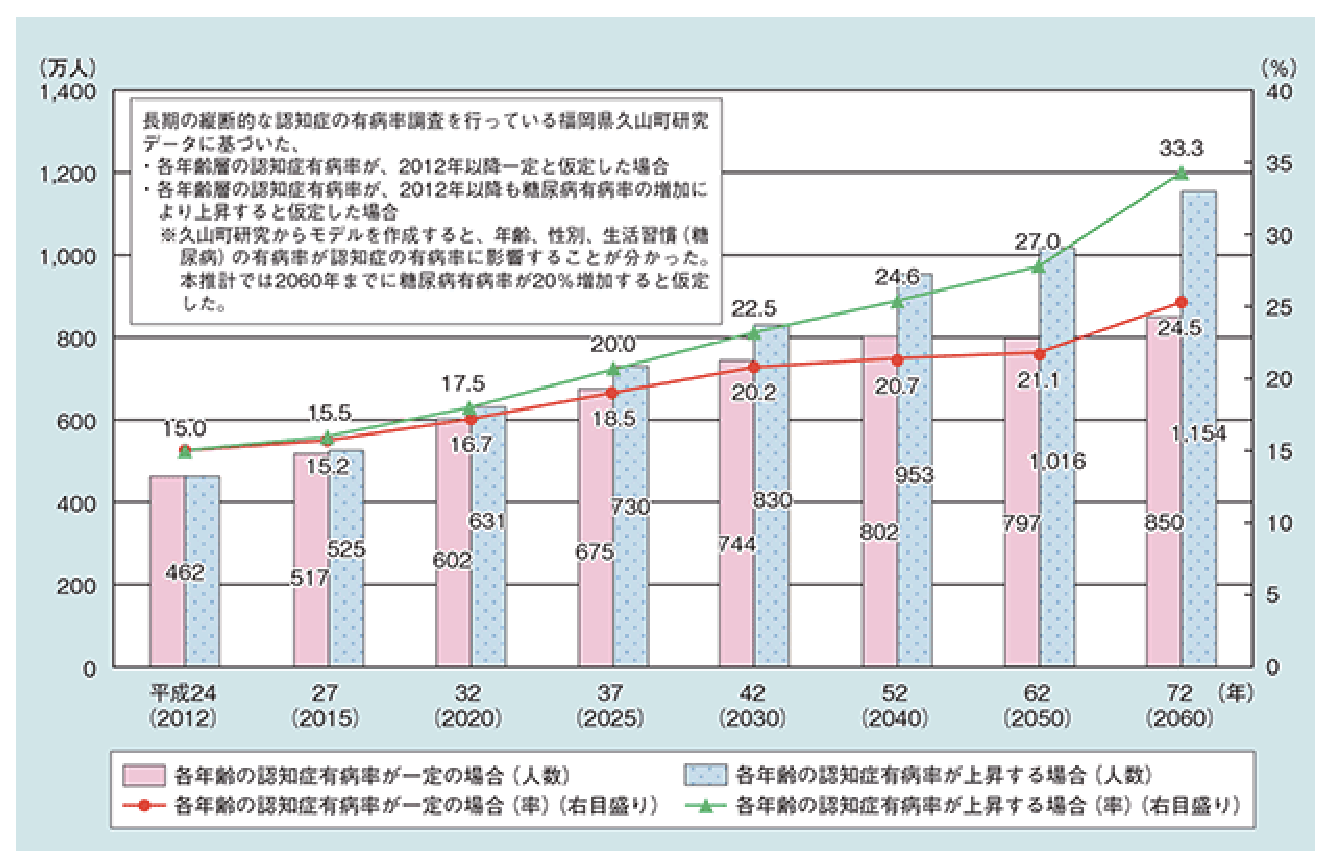
\includegraphics[width=0.9\textwidth]{chap1-figure/dementia_senior_number.eps}
	\caption{認知症高齢者数(文献\cite{高齢社会白書}より引用)}
	\label{fig:dementia_senior_number}
\end{figure}

\begin{figure}[tbp]
	\centering
			\includegraphics[width=0.9\textwidth]{chap1-figure/20171207_cognicise.eps}
	\caption{運動教室でのコグニサイズの実施の様子}
	\label{fig:20171207_cognicise}
\end{figure}

\begin{figure}[tbp]
	\centering
			\includegraphics[width=0.9\textwidth]{chap1-figure/cognistep.eps}
	\caption{コグニステップの実施方法(文献\cite{認知症予防へ向けた運動コグニサイズ}より引用)}
	\label{fig:cognistep}
\end{figure}


\if0
\begin{figure}[tbp]
	\centering
			\includegraphics[width=0.9\textwidth]{chap1-figure/rihabiri.eps}
	\caption{下肢リハビリ風景}
	\label{fig:rihabiri}
\end{figure}

\begin{figure}[tbp]
	\centering
			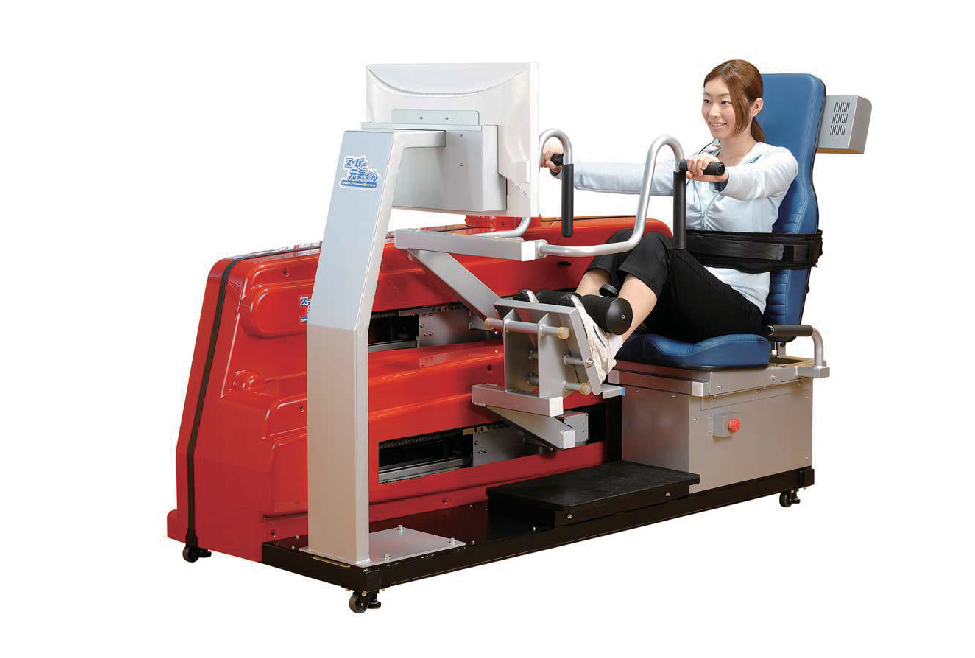
\includegraphics[width=0.9\textwidth]{chap1-figure/s-1.eps}
	\caption{下肢リハビリ器具正面図(文献\cite{フィットネスマシン}より引用)}
	\label{fig:smart-1}
\end{figure}

\begin{figure}[tbp]
	\centering
			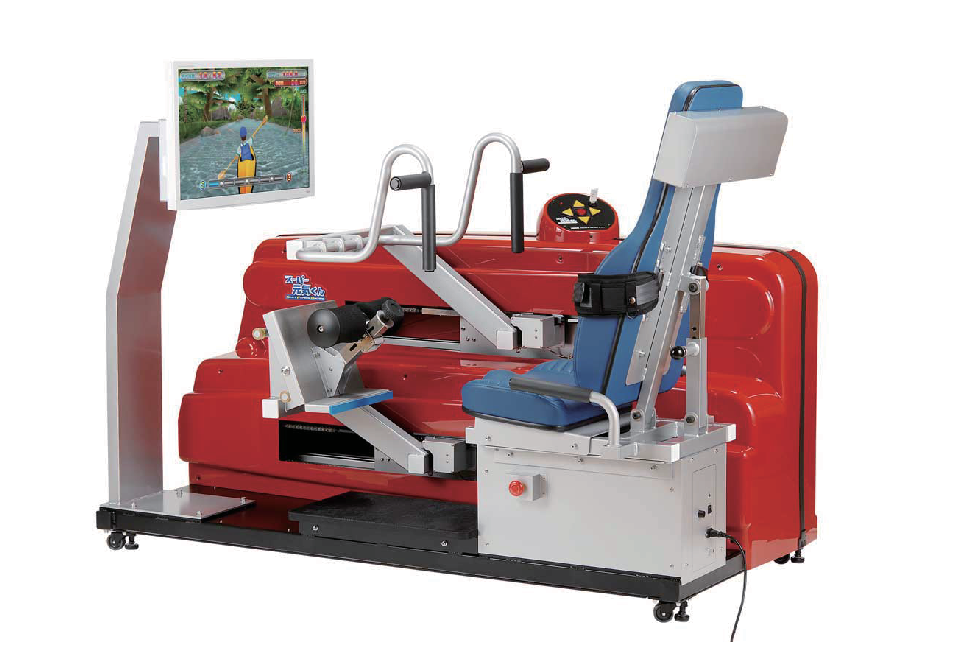
\includegraphics[width=0.9\textwidth]{chap1-figure/s-2.eps}
	\caption{下肢リハビリ器具側面図(文献\cite{フィットネスマシン}より引用)}
	\label{fig:smart-2}
\end{figure}

\begin{figure}[tbp]
	\centering
			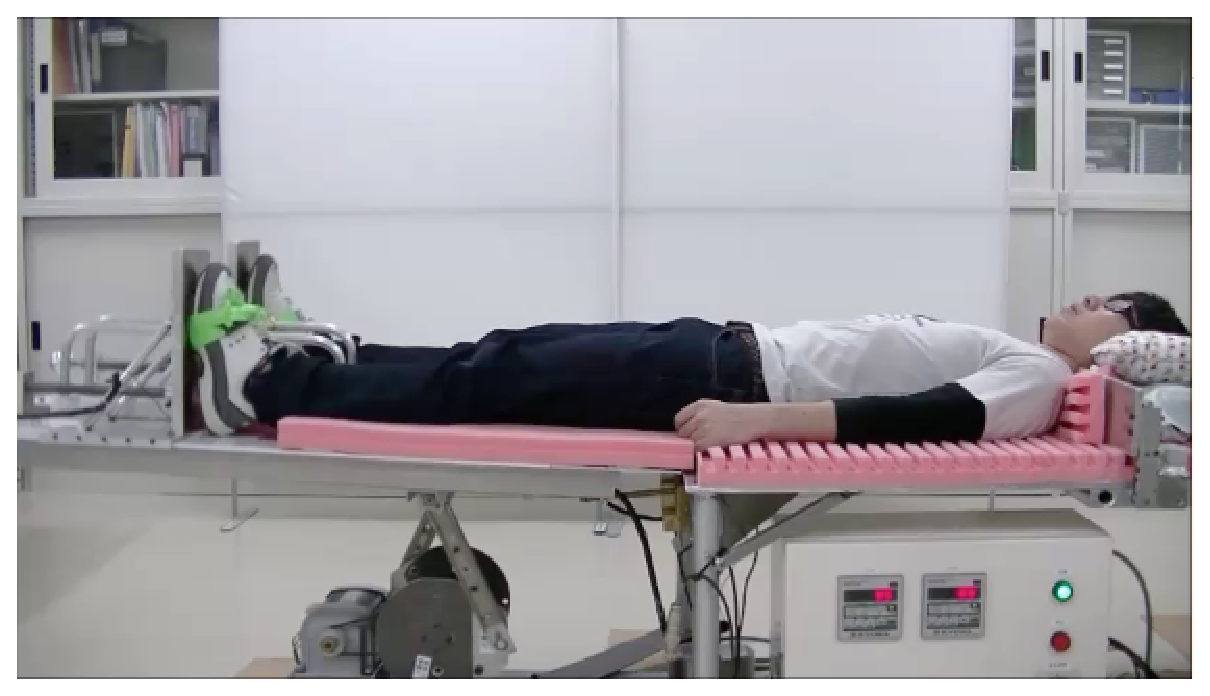
\includegraphics[width=0.9\textwidth]{chap1-figure/tadouhoku.eps}
	\caption{ベット型下肢リハビリ器具}
	\label{fig:tadouhokou}
\end{figure}

\begin{figure}[tbp]
	\centering
			\includegraphics[width=0.7\textwidth]{chap1-figure/Oculus.eps}
	\caption{HMD}
	\label{fig:Oculus}
\end{figure}
\fi

\section{関連研究}

\if0
本節では,機械を使用した下肢リハビリに関する研究と歩行感覚提示装置に使用するディスプレイに関する印象調査に関連する研究について述べる.維持期脳卒中患者に対して歩行感覚提示装置を用いた歩行トレーニングを行い,その効果の持続性の検討\cite{筑波歩行感覚提示}が田中らによって行われている.棚からの歩行感覚提示装置を図\ref{fig:tukuba}に示す.歩行感覚提示装置は,通常の歩行に近い動作かつ,通常の歩行と同じ1m/sの歩行速度を実現可能な装置である.患者は球面型ディスプレイ内を歩く構造となっている.入院前の健康状態の歩幅で自宅付近を歩く疑似体験をすることで,患者自身が早く治したいという気持ちになり,リハビリに対するモチベーションが向上するという精神面での効果も報告されている.しかし,寝たきりの患者は対象とされていない問題点がある.
\fi

\if0
\begin{figure}[tbp]
	\centering
			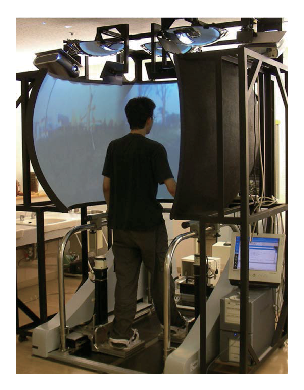
\includegraphics[width=0.5\textwidth]{chap1-figure/tukuba.eps}
	\caption{没入型歩行感覚提示装置全景(文献\cite{筑波歩行感覚提示画像}より引用)}
	\label{fig:tukuba}
\end{figure}

高齢者の自立・社会参加の前提となる歩行機能および歩行訓練に着目し,バーチャルリアリティ(VR: Virtual Reality)を活用した歩行訓練器具\cite{日立}が藤江らによって開発されている.藤江らによる歩行訓練機器を図\ref{fig:hitachi}に示す.リハビリ患者の歩行機能の改善を目指し,自立歩行によって実写映像が切り替わるシステムとなっている.VRを活用しリハビリ患者の訓練意欲を高める試みがされている.リハビリ患者に対して,立体視可能な映像を流した結果,映像に集中していたという結果が報告されている.そのことから,HMDを使用することがリハビリへの集中に繋がることも期待される.

\begin{figure}[tbp]
	\centering
			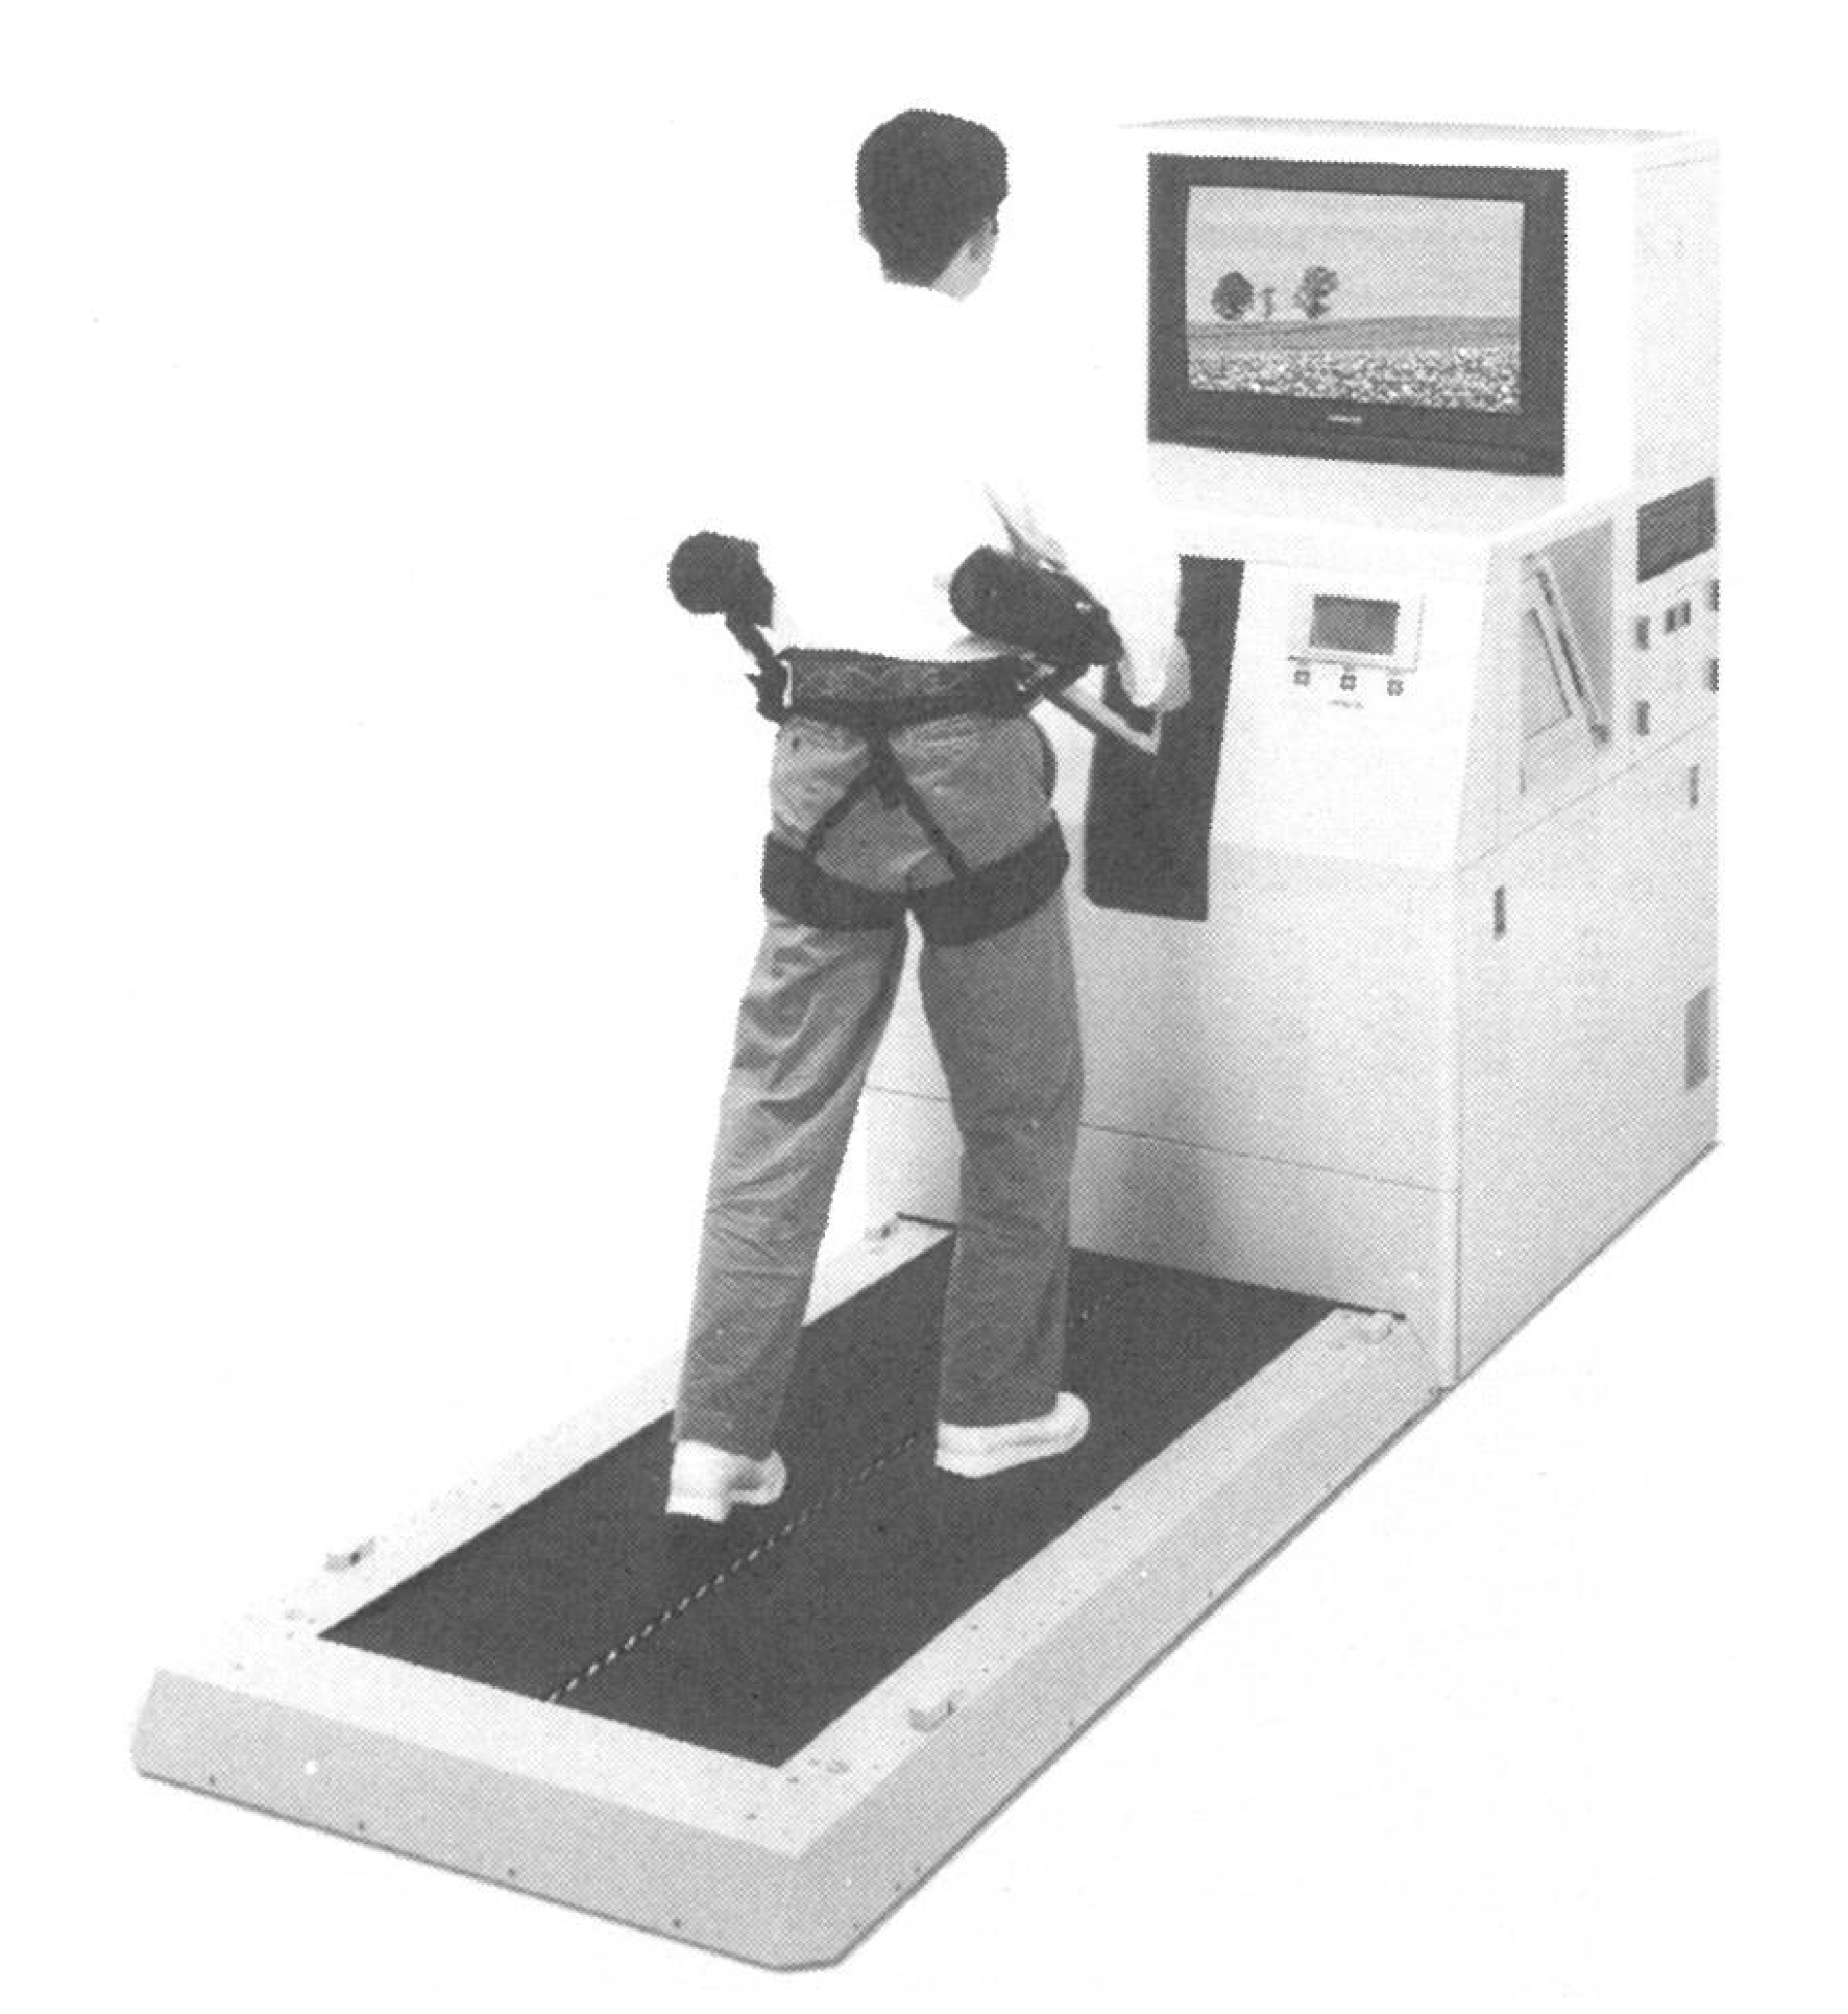
\includegraphics[width=0.5\textwidth]{chap1-figure/VRhokou.eps}
	\caption{バーチャルリアリティを活用した歩行訓練機器(文献\cite{日立}より引用)}
	\label{fig:hitachi}
\end{figure}

歩行感覚提示に使用するディスプレイの印象評価\cite{ディスプレイの違い}が小林らによって報告されている.ロコモーション・インターフェース\cite{ロコモーション}(LI: Locomotion Interface)を提示するディスプレイとして,プラズマディスプレイとHMDとスクリーンの3タイプのディスプレイを用い,ユーザに与える感覚を測定し分析が行われている.ロコモーション・インターフェースとは,VRにおいて,あたかも現実で歩いているような感覚を体感できる装置である.小林らの調査の結果,ディスプレイの違いによってユーザの感覚に差は僅差であったと報告されている.そのことから,ベッド型の下肢リハビリ装置には,着脱可能なHMDの利用が容易であると考えられる.

いずれの関連研究も自立で立ち上がることが可能なリハビリ患者を対象としており,寝たきりの患者は対象とされていない.
そこで本研究では,寝たきりの患者も対象とし,下肢リハビリを行う際の退屈さや歩行の想像の助けを行うシステムの開発をする.
\fi

\section{本研究の目的}
本研究では,ICTを使用し,運動教室で実施される集団でのコグニサイズにおいて,認知課題の負荷を個別に調整する支援を行うことを目的とする.認知課題の正答率を蓄積し,蓄積した認知課題の正答率に応じて,認知課題の負荷を調整可能なシステムを開発する.運動教室の参加者が提案システムを使用することによって,個別に認知症予防の効果があるコグニサイズを実施できることが期待される.

\section{論文の構成}
本稿の構成について述べる.第2章では提案システムの概要と処理の流れについて述べ,第3章では,評価を行う.そして,評価の結果からの考察を述べる.第4章では,以上で述べたことをまとめ,実験の考察の課題に基づき今後の課題を明らかにする.

\if0
本稿の構成について述べる.第2章では提案システムの概要と処理の流れについて述べ,第3章では,提案システムに関するSD法を使用したアンケートと記述式のアンケートで印象の評価を行う.そして,評価の結果からの考察を述べる.第4章では,以上で述べたことをまとめ,実験の考察の課題に基づき今後の課題を明らかにする.
\fi

% Local Variables: 
% mode: japanese-LaTeX
% TeX-master: "root"
% End: 
